\documentclass{article}
\usepackage{amsmath, amssymb}
\usepackage[retainorgcmds]{IEEEtrantools}
\usepackage{filecontents}
\usepackage{hyperref}
\usepackage{graphicx}
\author{Derek Kuo, Henry Milner}
\title{CS267 HW2: Particle Simulation}
\date{3/13/15}

% Some functions for general use.

\newcommand{\code}[1]%
  {\texttt{#1}}

\def\seqn#1\eeqn{\begin{align}#1\end{align}}

\newcommand{\vecName}[1]%
  {\boldsymbol{#1}}

\newcommand{\io}%
  {\text{ i.o. }}

\newcommand{\eventually}%
  {\text{ eventually }}

\newcommand{\tr}%
  {\text{tr}}

\newcommand{\Cov}%
  {\text{Cov}}

\newcommand{\adj}%
  {\text{adj}}

\newcommand{\funcName}[1]%
  {\text{#1}}

\newcommand{\hasDist}%
  {\sim}

\DeclareMathOperator*{\E}%
  {\mathbb{E}}

\newcommand{\Var}%
  {\text{Var}}

\newcommand{\std}%
  {\text{std}}

\newcommand{\grad}%
  {\nabla}

\DeclareMathOperator*{\argmin}{arg\,min}

\DeclareMathOperator*{\argmax}{arg\,max}

\newcommand{\inprod}[2]%
  {\langle #1, #2 \rangle}

\newcommand{\dd}[1]%
  {\frac{\delta}{\delta#1}}

\newcommand{\Reals}%
  {\mathbb{R}}

\newcommand{\indep}%
  {\protect\mathpalette{\protect\independenT}{\perp}} \def\independenT#1#2{\mathrel{\rlap{$#1#2$}\mkern2mu{#1#2}}}

\newcommand{\defeq}%
  {\buildrel\triangle\over =}

\newcommand{\defn}[1]%
  {\emph{Definition: #1}\\}

\newcommand{\example}[1]%
  {\emph{Example: #1}\\}

\newcommand{\figref}[1]%
  {\figurename~\ref{#1}}

\newtheorem{theorem}{Theorem}[section]
\newtheorem{lemma}[theorem]{Lemma}
\newenvironment{proof}[1][Proof]{\begin{trivlist}
\item[\hskip \labelsep {\bfseries #1}]}{\end{trivlist}}

\begin{filecontents}{\jobname.bib}
@inproceedings{graphlab,
  title = {GraphLab: A New Parallel Framework for Machine Learning},
  author = {Yucheng Low and
            Joseph Gonzalez and
            Aapo Kyrola and
            Danny Bickson and
            Carlos Guestrin and
            Joseph M. Hellerstein},
  booktitle = {Conference on Uncertainty in Artificial Intelligence (UAI)},
  month = {July},
  year = {2010}
}
@inproceedings{graphx,
  title={Graphx: A resilient distributed graph system on spark},
  author={Xin, Reynold S and Gonzalez, Joseph E and Franklin, Michael J and Stoica, Ion},
  booktitle={First International Workshop on Graph Data Management Experiences and Systems},
  pages={2},
  year={2013},
  organization={ACM}
}
@inproceedings{mapgraph,
  author = {Fu, Zhisong and Personick, Michael and Thompson, Bryan},
  title = {MapGraph: A High Level API for Fast Development of High Performance Graph Analytics on GPUs},
  booktitle = {Proceedings of Workshop on GRAph Data Management Experiences and Systems},
  series = {GRADES'14},
  year = {2014},
  isbn = {978-1-4503-2982-8},
  location = {Snowbird, UT, USA},
  pages = {2:1--2:6},
  articleno = {2},
  numpages = {6},
  url = {http://doi.acm.org/10.1145/2621934.2621936},
  doi = {10.1145/2621934.2621936},
  acmid = {2621936},
  publisher = {ACM},
  address = {New York, NY, USA},
  keywords = {GPU, Graph analytics, high-level API},
}
@inproceedings{durand2012packed,
  title={A Packed Memory Array to Keep Moving Particles Sorted},
  author={Durand, Marie and Raffin, Bruno and Faure, Fran{\c{c}}ois},
  booktitle={9th Workshop on Virtual Reality Interaction and Physical Simulation (VRIPHYS)},
  pages={69--77},
  year={2012},
  organization={The Eurographics Association}
}
\end{filecontents}

\begin{document}
\maketitle

\section{Introduction}
For this assignment, we have implemented several versions of a 2D particle simulator.  We describe our implementations and their performance, and close with some comments.  First, let us describe the problem and a general framework for solutions.

We simulate a system of particles interacting in a 2D square box.  Particles can bounce off each other or the walls of the box.  The size of the box is scaled so that the average density of particles is constant as the number of particles, $n$, increases.  The particles are initialized with bounded random velocity.

The simulator for this assignment discretizes time into $T = 1000$ time steps and defines inter-particle interactions such that each particle interacts only with other particles within a bounded radius on each time step.  On each time step, it uses a two-step algorithm: First, forces from other nearby particles determine the particle's acceleration.  Then, each particle moves according to its current acceleration and velocity, bouncing inelastically off walls as necessary.  We call the first step ``interaction'' and the second step ``movement''.

Our goal is to implement this simulation algorithm as quickly as possible, either by eliminating unnecessary work or by parallelizing the computation across $p$ hardware threads.  Clearly a lower bound on running time is $O(T n / p)$, since each particle must be touched on each time step.  Movement takes $O(n)$ time and is perfectly parallel.  (For that reason, we will not discuss how we implement the movement step, except where it could be unclear.)  However, a naive algorithm does $O(n^2)$ work in the interaction step, and it is unclear how to parallelize it efficiently.

The general trick for speeding up the interaction step will be to maintain a data structure that allows us to query only a small number of nearby particles (say $K$) for each particle in the second step, reducing the running time to $O(Kn)$.  If $K$ is constant, then we have achieved $O(n)$ running time, which is the best asymptotic running time for this problem (assuming we must implement the simulation algorithm exactly, up to reordering floating-point operations).  To parallelize the interaction step, we must ensure that these $Kn$ queries do not involve too much communication, and that we can parallelize the maintenance of the data structure itself.  There is a generic data structure to solve the former problem, so often the difficult part is maintaining the data structure efficiently.

\subsection{Experimental setup}
We run our experiments in three different computing environments.  Most experiments are run on the Hopper cluster.  Experiments on GPUs are run on Stampede nodes.  When noted, we also run experiments on a Mid-2012 Macbook Pro, which has an NVIDIA GeForce GT 650M GPU with 1GB of memory and a 2.3 GHz Core i7 CPU.

\section{Serial Implementation}
Our serial implementation uses a grid data structure to execute the interaction step in $O(n)$ time.  The box is divided into $O(n)$ equal squares (approximately $n$ squares in our implementation), which are large enough that a particle can only interact with particles in its own square and its 8 neighboring squares on a single iteration.  Squares are stored in a flat vector in column-major order, and each square contains a pointer to a vector of pointers to the particles it currently contains.  In the interaction step, each particle only needs to be checked for interactions with particles in 9 squares; since the number of particles per square is bounded (and equal to 1 on average), the interaction step takes $O(n)$ time.  After the movement step, particles must be mapped to new grid squares, so we simply build a new grid serially, which takes $O(n)$ time.

\subsection{Results}
Figure \ref{fig:serial-on} shows that our algorithm indeed enjoys linear ($O(n)$) scaling.  For comparison, Figure \ref{fig:serial-naive} shows the performance of the naive $O(n^2)$ algorithm on smaller problems.

We also ran our experiments on our laptop, and the laptop runs the serial code faster than the Hopper nodes, which are not designed for serial performance.  Figure \ref{fig:serial-laptop} shows the results; the laptop does slightly outperform Hopper.

\begin{figure}
  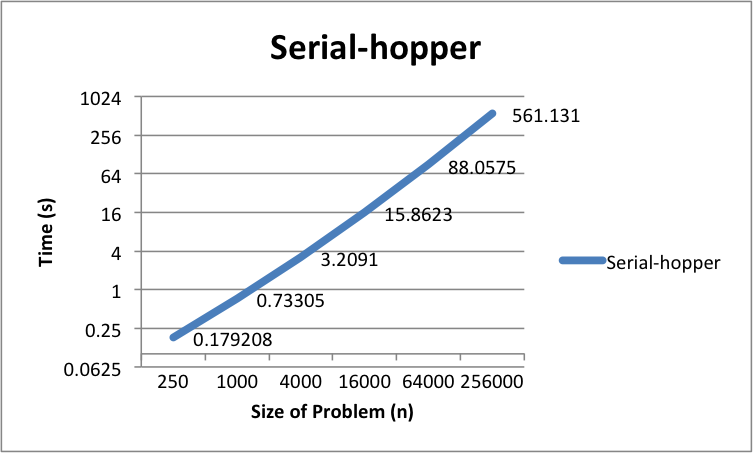
\includegraphics[width=\textwidth]{plots/Serial-Hopper.png}
  \caption{$O(n)$ scaling of the serial algorithm.}
  \label{fig:serial-on}
\end{figure}

\begin{figure}
  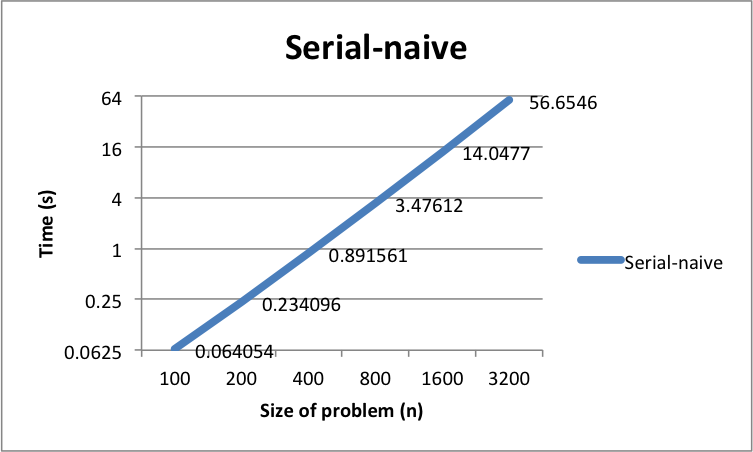
\includegraphics[width=\textwidth]{plots/Serial-Naive.png}
  \caption{Performance of the $O(n^2)$ serial algorithm.}
  \label{fig:serial-naive}
\end{figure}

\begin{figure}
  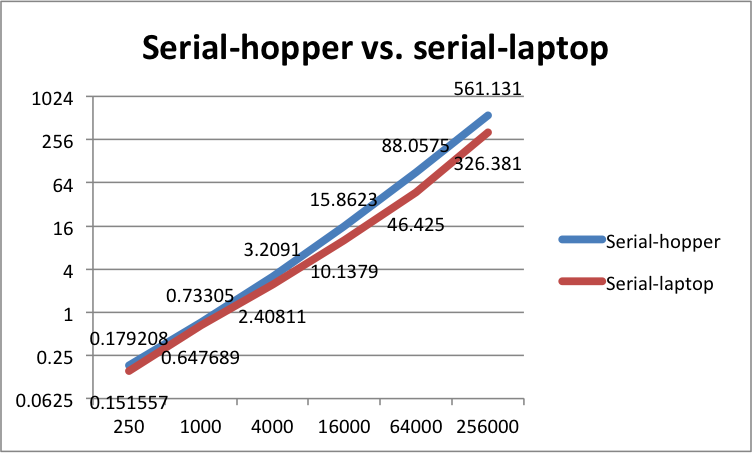
\includegraphics[width=\textwidth]{plots/Serial-laptop-vs-hopper.png}
  \caption{Performance of the serial algorithm on Hopper and a laptop.  (Running time is the on the y axis, and problem size is on the x axis.  Smaller is better.)}
  \label{fig:serial-laptop}
\end{figure}

\section{OpenMP Implementation}
Our OpenMP implementation uses a similar grid data structure.  To maximize cache locality, each thread is assigned a block of grid squares whose particles' accelerations it must compute in the interaction step.  With this scheme, a thread needs only read particles from its own squares and from squares bordering its block.  The grid itself is also built in parallel.  After movement, each thread inserts into a new shared grid data structure all the particles that were in its block before movement.  Each square uses a separate \code{omp\_lock\_t} to ensure that inserts are atomic.

In principle, we should use a block structure that minimizes the maximum border size.  If $p$ is a perfect square, an optimal block structure consists of squares of grid squares; since there are $O(n)$ total squares, the maximum border size is $O((n/p)^{1/2})$.  However, due to time constraints, we used a less efficient block structure, just a range of grid squares in column major order.  This results in a larger border size of $O(\min(n/p, \sqrt{n}))$.

\subsection{Synchronization}
Finally, let us describe the details of synchronization in this algorithm.  In pseudocode, the algorithm looks like this:

\begin{verbatim}
particle_t* particles = makeSystem() # O(n), done on 1 thread
Grid oldGrid
Grid newGrid = buildInitially(particles) # O(n), done on 1 thread
for i in range(1, T):
  barrier()
  oldGrid = newGrid # O(1), done on 1 thread
  newGrid = new Grid() # O(1), done on 1 thread
  barrier()
  insertIntoGrid(oldGrid, newGrid) # Done in parallel using locks
  barrier()
  simulateInteractions(newGrid) # Done in parallel
  barrier()
  simulateMovements(newGrid) # Done in parallel

def insertIntoGrid(oldGrid, newGrid):
  parfor square in oldGrid: # thread j handles block of squares j
    for particle in square:
      lock(locks[destinationSquareIndex(particle)])
      insert(particle, newGrid.destinationSquare(particle))
      unlock(locks[destinationSquareIndex(particle)])
\end{verbatim}

\begin{description}
  \item[Interactions:] Since each particle's acceleration is written by only a single thread in the \code{simulateInteractions} step, no synchronization is required within that step.
  \item[Building the grid:] \code{insertIntoGrid} does require synchronization, since a grid square can have particles inserted into it by multiple threads at once.  We use fine-grained locking on inserts using a separate \code{omp\_lock\_t} for each grid square.
  
  There is a potential problem with our implementation here: The OMP spec says that locked sections are protected by global memory barriers, when we really only want a memory barrier on the grid square that has been locked.  This means that the OMP runtime may do much more communication than necessary when running our algorithm.  Our implementation has performance problems that could be caused by this.  If we had more time, we would investigate whether this was the cause.
  
  Note that we always insert into a new copy of the grid, rather than moving particles within a grid.  The latter approach would be vulnerable to race conditions without careful synchronization, since it involves mixed deletes and inserts of particles.  Using a new grid ensures that \code{insertIntoGrid} is a monotonic operation, which makes it relatively easy to parallelize.  
  \item[Movements:] A barrier is required between \code{simulateInteractions} and \code{simulateMovements} to ensure that particles in a thread's border do not move before it can include them in an interaction.
  \item[Initialization:] The initialization step takes $O(n)$ time and is not parallelized.  The assignment says this is okay, but in a real system we would want to parallelize this step.
\end{description}

\subsection{Results}
Figure \ref{fig:openmp-on} shows that our algorithm scales linearly with problem size, for $p=1$ or $p=24$ threads.  Figure \ref{fig:openmp-weak} shows weak scaling: We increase the number of threads, increasing $n$ proportionally, for various base problem sizes.  Our algorithm does not enjoy weak scaling; a least-squares fit of log-performance against $\alpha \log n$ gives $\alpha \approxeq 1/2$ for large $n$, indicating that the asymptotic performance could be $O(n/\sqrt{p})$.  Figure \ref{fig:openmp-strong} gives similarly bad news for strong scaling.

\begin{figure}
  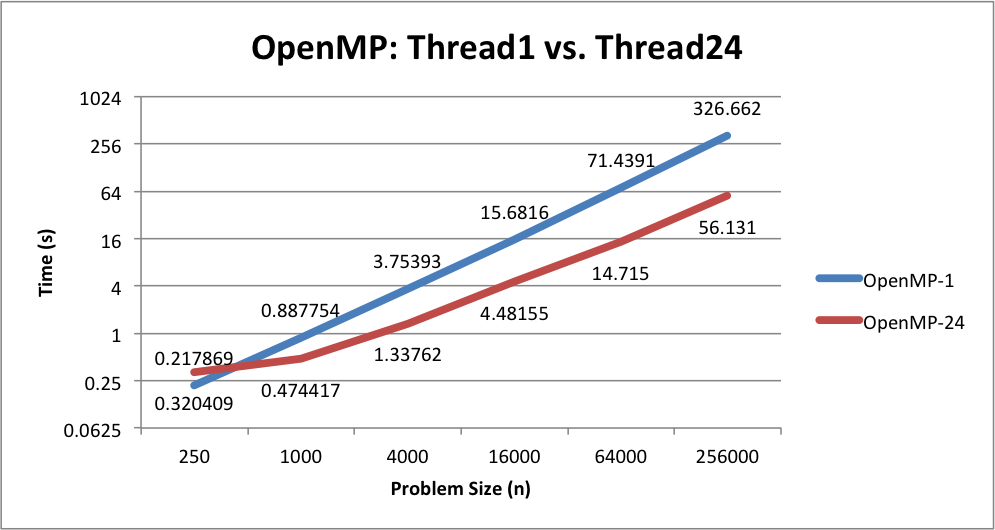
\includegraphics[width=\textwidth]{plots/OpenMP-Thread1-vs-Thread24.png}
  \caption{$O(n)$ scaling of the OpenMP implementation using $1$ and $24$ threads.}
  \label{fig:openmp-on}
\end{figure}

\begin{figure}
  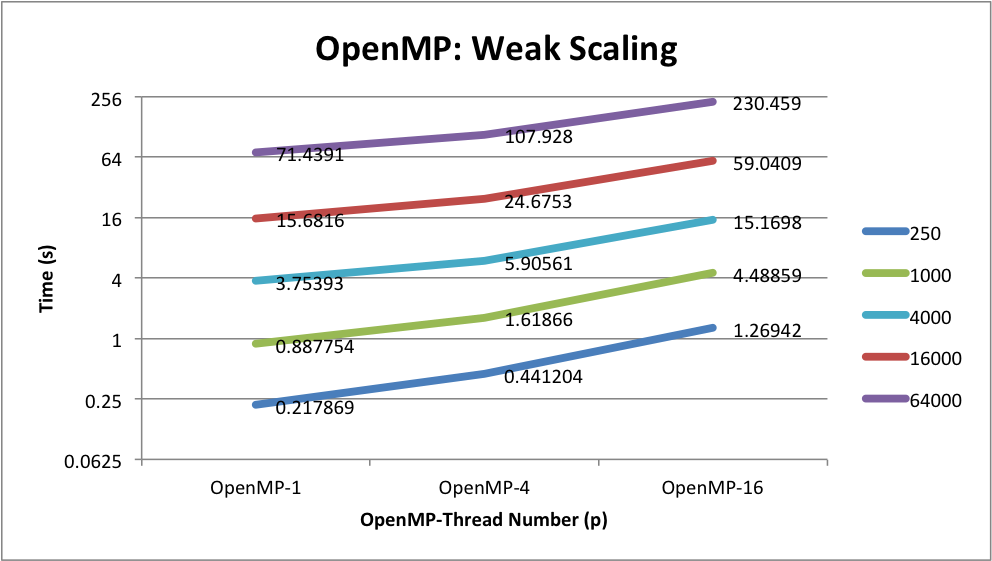
\includegraphics[width=\textwidth]{plots/OpenMP-weak-scaling.png}
  \caption{Weak scaling of the OpenMP implementation, for various base problem sizes.}
  \label{fig:openmp-weak}
\end{figure}

\begin{figure}
  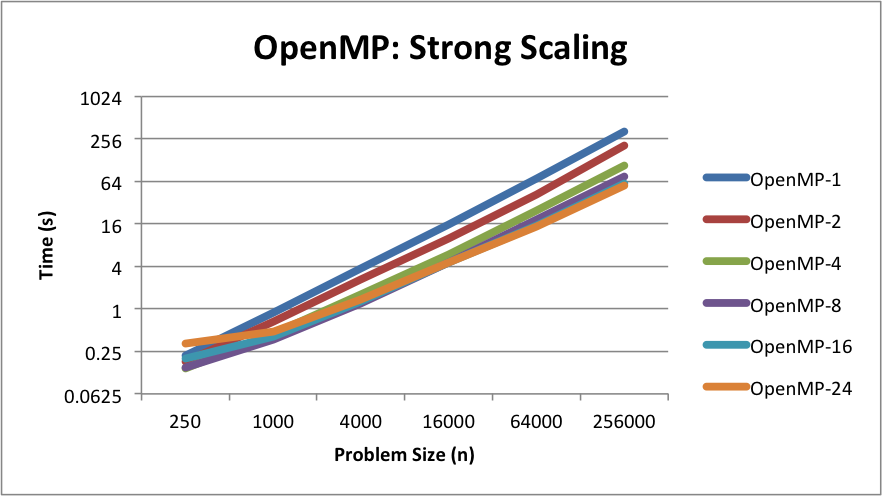
\includegraphics[width=\textwidth]{plots/OpenMP-Strong-scaling.png}
  \caption{Strong scaling of the OpenMP implementation, for various base problem sizes.}
  \label{fig:openmp-strong}
\end{figure}

\section{MPI Implementation}
Our MPI implementation centered on three parts: (1) the division of particle regions for each node - how over all particles are divided and handled; (2) the communication and message format passing among each node - what different type of information are passed through MPI commands; and (3) the faster $O(n)$ algorithm achieved by grids.

\subsection{The division of particles}
Initially, the master node (rank=0) scans all of the particles and assigns them to a processor based on their locations in the box. Based on the number of nodes specified by the user, the program equally divides the region into subregion administrated by each node. In its own region, the node calculates forces and moves particles based on local data. A node holds two types of local data: (1) particles inside the region (2) particles outside the region but in the boundary of squares immediately around the region. With this local data, each node has sufficient information to calculate its own particles' movements.

\subsection{Communication between nodes}
After applying forces and movements, each particle has a new coordinate. Each node checks whether its particles have (1) moved outside the region; (2) stayed inside the region but at the boundary of other nodes; or (3) stayed inside the region and not at boundary. The node then use \code{MPI\_Isend()} and \code{MPI\_Recv()} to communicate with other nodes and send the list of type (1) and type (2) particles to the exact nodes they should received. One thing to note is we are using non-blocking \code{MPI\_Isend()} and blocking \code{MPI\_Recv()} to avoid deadlock.

\subsection{Faster algorithm with grid}
Similar to OpenMP, the MPI implementation uses a grid data structure to improve the time efficiency to $O(n)$. However, instead of shared grid structure, each node maintains its own local grid. In principle, we could use an $O(n^2)$ algorithm locally, if the subproblem solved by each node were too small to justify the overhead of maintaining a grid.  In practice, it is better to use the linear algorithm.

\subsection{pseudocode}

\begin{verbatim}
For each step within each node:
  ApplyForce(innerParticles, localGrid)
  ApplyForce(innerParticles, boundryParticles)
  Move(innerParticles)
  ScanParticles(innerParticles)
  CommunicateOutside(outsideParticlesAfterMove)
  CommunicateBoundryParticle(boudryParticlesAfterMove)
  ReceiveOutsideParticles(outsideBuf)
  ReceiveBoundryParticles(boundryBuf)
  UpdateInnerParticles(outsideBuf)
  UpdateLocalGrid(outsidebuf)
  
\end{verbatim}

\subsection{Results}
Figure \ref{fig:mpi-on} shows that our algorithm scales linearly with problem size, for $p=1$ or $p=16$ nodes.  Figure \ref{fig:mpi-weak} shows weak scaling: We increase the number of nodes, increasing $n$ proportionally, for various base problem sizes.  Our MPI algorithm enjoys better weak scaling, although not perfect.  Figure \ref{fig:mpi-strong} shows a similar situation for strong scaling.

\begin{figure}
  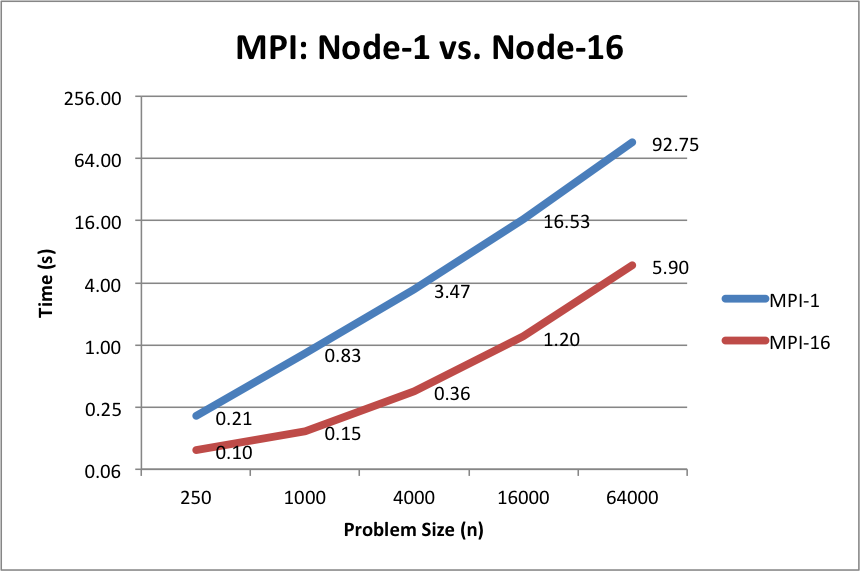
\includegraphics[width=\textwidth]{plots/MPI-node1-vs-node16.png}
  \caption{$O(n)$ scaling of the MPI implementation using $1$ and $16$ nodes.}
  \label{fig:mpi-on}
\end{figure}

\begin{figure}
  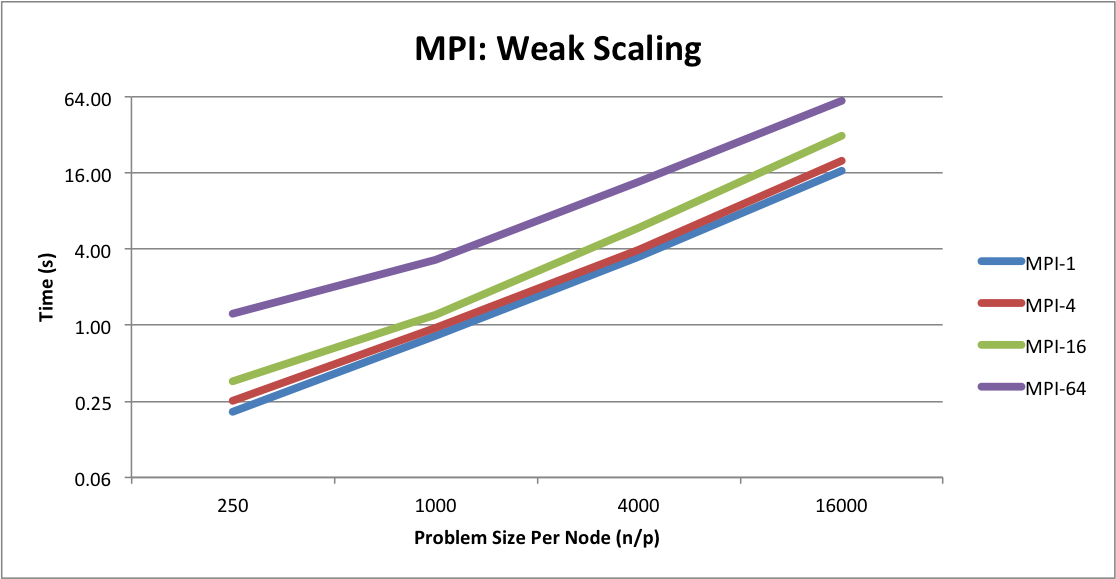
\includegraphics[width=\textwidth]{plots/MPI-weak-scaling.png}
  \caption{Weak scaling of the MPI implementation, for various base problem sizes.}
  \label{fig:mpi-weak}
\end{figure}

\begin{figure}
  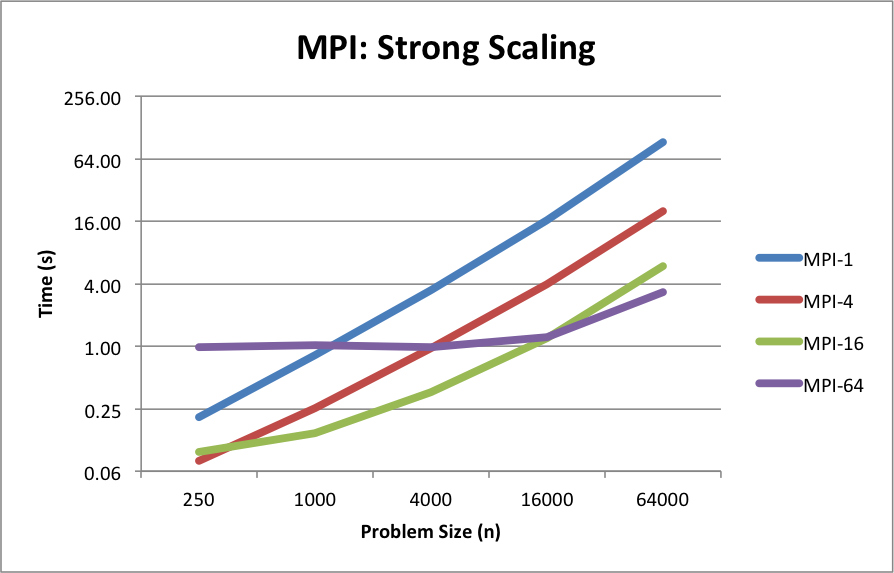
\includegraphics[width=\textwidth]{plots/MPI-strong-scaling.png}
  \caption{Strong scaling of the MPI implementation, for various base problem sizes.}
  \label{fig:mpi-strong}
\end{figure}

\section{CUDA Implementation}
Our CUDA implementation is similar to our others, except for the step that builds the grid data structure.  In our other code, each grid square is a pointer to a dynamic array of pointers to a global list of particles.  This means that inserting into the grid requires dynamic allocation of memory and locking, both of which are purportedly expensive on the GPU.  Instead, we store particles in a flat array, sorted by grid square location in column-major order.  A separate array stores pointers from grid square index to the first particle contained in the grid square.  This allows us to use Thrust's efficient implementation of \code{sort()} to rebuild the grid.

Pseudocode for the relevant parts of our algorithm (slightly cleaner than what is actually needed to implement this in Thrust) looks like this:

\begin{verbatim}
for i in range(1, T):
  rebuildGrid(particles, gridPointers)
  simulateInteractions(particles, gridPointers)
  simulateMovements(particles)
  
def rebuildGrid(particles, gridPointers):
  newGridIndices = particles.map(destinationSquareIndex)
  particles.sortByKey(newGridIndices, particles)
  # Now compute the grid offsets from the sorted particles:
  newGridCounts = newGridIndices.map(i => (i, 1)).reduceByKey(0, +)
  padWithZeros(newGridCounts) # Ensure that any empty grid squares are indexed.
  newGridOffsets = newGridCounts.exclusiveScan(0, +)
\end{verbatim}

Each of the steps in \code{rebuildGrid} can be implemented using only constant memory that is preallocated in the GPU.  Thrust's \code{sort()} has a reputation for being highly optimized, so it is possible that it would be hard to beat our implementation without heavy optimization.  However, since we use a generic sorting algorithm, we do pay an additional $\log(n)$ factor on each iteration, so that our algorithm technically runs in $O(T n \log n)$ time.  This seems to be irrelevant for all problem sizes that would fit into GPU memory on the machines we used -- the code actually scales sublinearly.  Still, we will discuss some potential improvements in Section \ref{sec:future}.

There is another way in which Thrust's mapreduce-like interface does not map well to this problem: Our implementation of \code{simulateInteractions} had to be done in raw CUDA (using essentially the same code as other parallel interaction steps) rather than using Thrust primitives.  Simulating interactions in mapreduce requires zipping each particle with its neighboring particles, but we could find no efficient or even natural way to do that in Thrust.  But it is nice that Thrust allows us to go back and forth between its vector abstraction and a raw block of device memory.

\subsection{Results}
Figure \ref{fig:gpu-on} shows that our implementation's runtime scales linearly with $n$.  (In fact, there seems to be a constant or $o(1)$ term in the runtime, since it scales slightly sublinearly.)  Figure \ref{fig:gpu-naive} compares our implementation with the naive algorithm; it is much faster than the naive $O(n^2)$ algorithm even for the smallest simulation size.  This suggests that using Thrust does not introduce any significant constant overhead, since the naive algorithm is simple, bare CUDA.

Finally, in Figure \ref{fig:gpu-laptop} we compare the performance of the NVIDIA K20 GPU with the Geforce GT 650M in a Macbook Pro.  The K20 is about 4 times as fast for the largest problem size, and it can handle much larger problems (it has 5 times as much memory, and the 650M was simultaneously driving a retina Macbook display).

\begin{figure}
  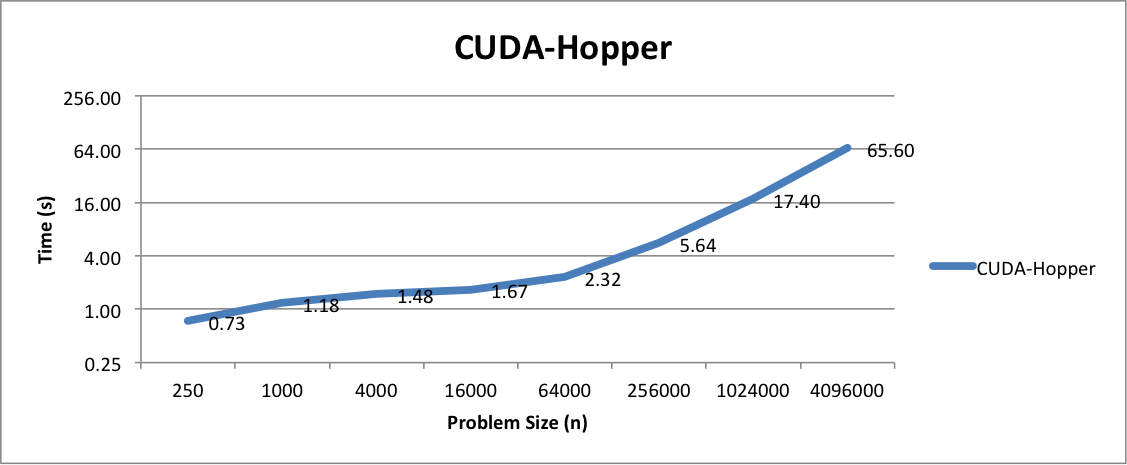
\includegraphics[width=\textwidth]{plots/CUDA-hopper.png}
  \caption{$O(n)$ scaling of the CUDA implementation.}
  \label{fig:gpu-on}
\end{figure}

\begin{figure}
  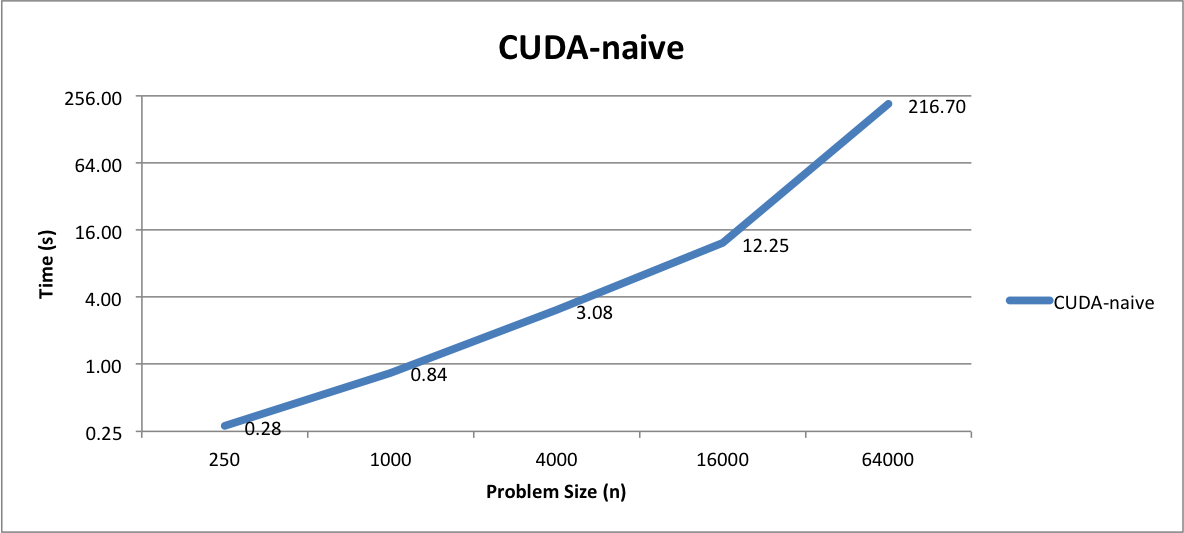
\includegraphics[width=\textwidth]{plots/CUDA-naive.png}
  \caption{Comparison of the CUDA implementation with the naive $O(n^2)$ version.}
  \label{fig:gpu-naive}
\end{figure}

\begin{figure}
  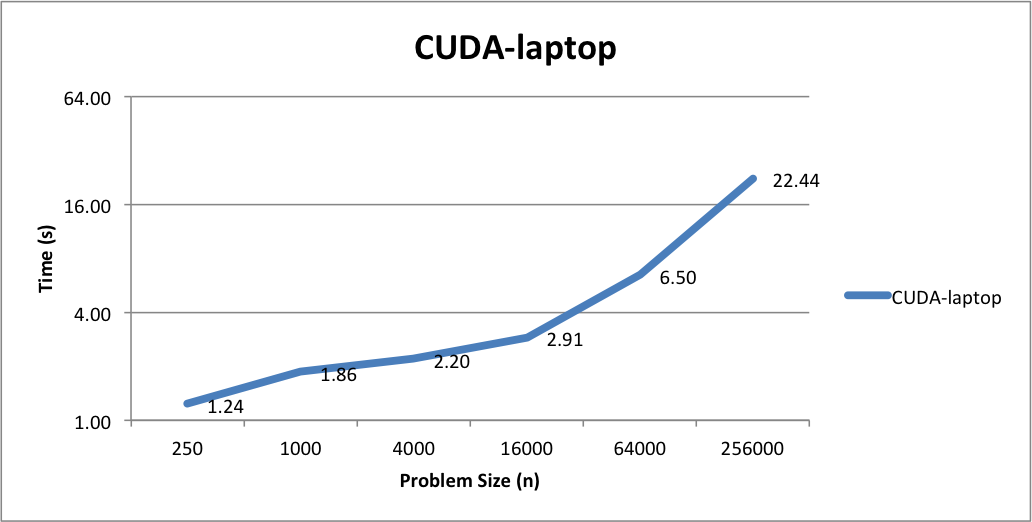
\includegraphics[width=\textwidth]{plots/CUDA-laptop.png}
  \caption{Comparison of CUDA code running on a laptop and on a Stampede node.}
  \label{fig:gpu-laptop}
\end{figure}

\section{Observations}
We close with some observations.

\subsection{Performance Comparison}
Figure \ref{fig:all} shows the performance of all the implementations we have discussed.  Some takeaways:
\begin{description}
  \item[Asymptotics are important:] The $O(n)$ algorithm beat the $O(n^2)$ algorithm at modest problem sizes -- at $n=250$ for serial code and at $n=4000$ for GPU code -- despite using more complex data structures.
  \item[GPUs win:] Running on Stampede, the GPU code beats all other implementations by a factor of roughly 3 for large problem sizes.  This is true even for MPI code running on 11 Hopper nodes.  GPU code running on a laptop is competitive with MPI code on a small cluster.  However, the GPU is limited by the availability of memory ($n=256000$ for the laptop and $n=16384000$ for Stampede), while the MPI code could presumably scale to even larger problems than we tested, albeit very slowly.  This limitation could potentially be lifted by swapping to machine memory, but that would diminish or eliminate the benefits of using the GPU.
\end{description}

\begin{figure}
  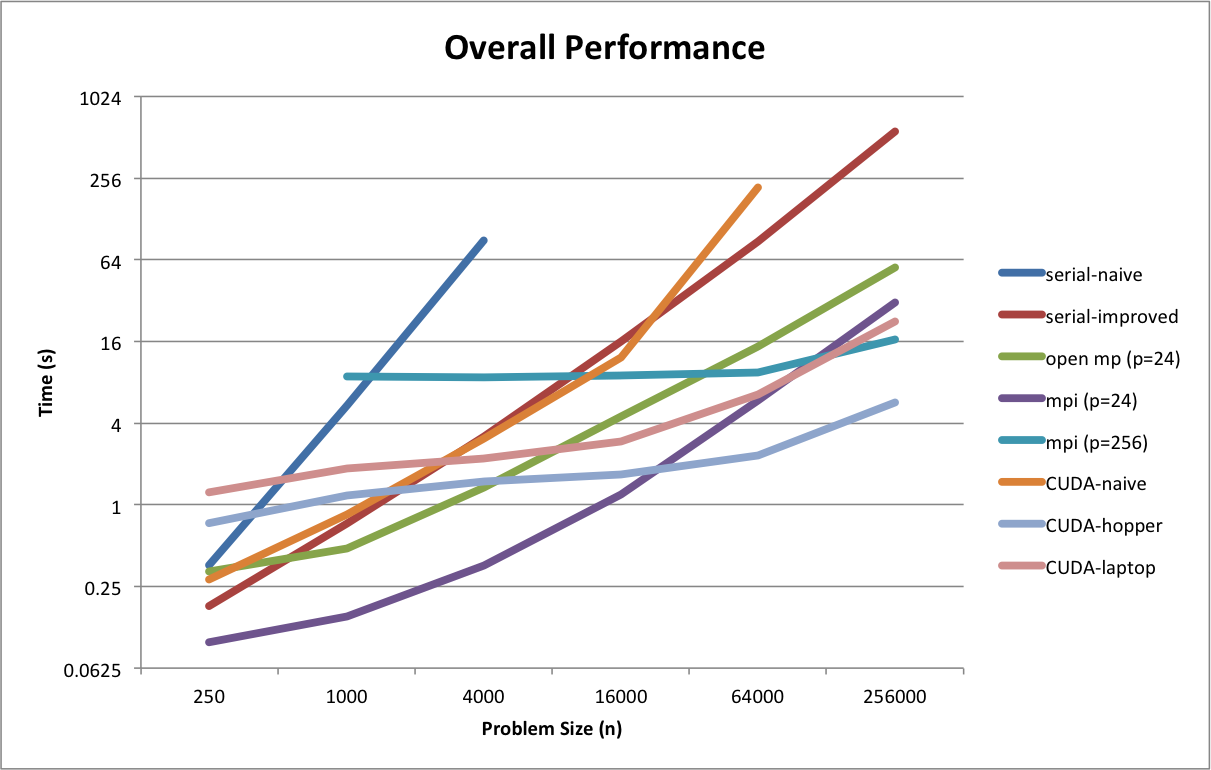
\includegraphics[width=\textwidth]{plots/Overall.png}
  \caption{Comparison of all particle simulator implementations.}
  \label{fig:all}
\end{figure}

\subsection{Future Work}
\label{sec:future}
None of the programming models we used in this project were perfectly suited to the problem.  In each case, it was difficult to minimize communication when building the grid data structure and using it to simulate particle interactions.  Instead, it seems best to think of particle simulation as a graph-parallel problem.  In every implementation we discretize the problem domain into squares; each square does bounded work (since the number of particles per square is bounded) and communicates particles and forces with a bounded number of neighbors on each iteration.  It is natural to think of the squares as nodes in a (dynamic) graph of bounded degree.  Systems like GraphLab \cite{graphlab} or GraphX \cite{graphx} therefore ought to provide an easy and efficient way to implement our particle simulator.  A recent system, MapGraph, could even be used to run on a GPU.  It would be interesting to investigate this.

Another interesting question raised by this assignment is: What is a better approach to reordering particles in the GPU code?  Thrust's \code{sort()} does not seem to introduce a noticeable bottleneck in practice, so this is largely an academic exercise.  But in theory, we have introduced an $O(n \log n)$ step in an algorithm that could run in $O(n)$ time.  We could fix this by using a sorting algorithm that (1) sorts in place, (2) sorts in parallel on a GPU, and (3) takes $O(M)$ time, where $M$ is the total distance traveled by particles from their original order.  In other words, we can take advantage of the fact that the list of particles stays \emph{nearly sorted} on each iteration.  (This is equivalent to the fact that the computation graph in GraphLab would be of bounded degree.)  There are two difficulties that may not be resolvable.  First, we know of no such sorting algorithm.  Second, we would need to sort on a one-dimensional embedding of the particles that ensures all neighboring particles, and not too many more particles on average, appear as neighbors (say, within $k$ places of the particle) in the sorted order.  We are not sure if such a scheme is possible.  (Locality-sensitive hashing is one potential method.)  There is some recent related work to explore: \cite{durand2012packed}.

\section{Notes on Running Our Code}
We used GNU g++ to compile all parts of our code (other than that compiled with nvcc).  On Hopper, please run \code{module swap PrgEnv-pgi PrgEnv-gnu} before attempting to run the build.  On Stampede, run \code{module load cuda} before building.

\bibliographystyle{plain}
\bibliography{\jobname}

\end{document}